\documentclass[11pt, a4paper]{article}
% Set the fonts of the document
\usepackage{inconsolata} % Monospace font
\usepackage{helvet} % Sans-serif font
\usepackage[
    libertine, % do not override the sans-serif-font
    tt = false % do not override the monospace font
]{libertine} % Main font (serif)

\usepackage[
    top = 3cm,
    bottom = 3cm,
    left = 2.5cm,
    right = 2.5cm
]{geometry}

\usepackage[english]{babel}
\usepackage{xspace}
\usepackage{booktabs}
\usepackage{enumitem}
\usepackage[xcolor]{mdframed}
\usepackage{amsmath}
\usepackage{amssymb}
\usepackage{amsthm}
\usepackage{mathrsfs}
\usepackage{stmaryrd}
\usepackage{float}
\usepackage{listings}
\usepackage{parskip}
\usepackage[
    labelfont = {small, bf},
    textfont = {small}
]{caption}
\usepackage{subcaption}
\usepackage{circledsteps}
\usepackage{hyperref}

% ====================================================================

\newcommand{\eg}{e.g.,\xspace}
\newcommand{\ie}{i.e.\xspace}
\newcommand{\etal}{\textit{et~al.}\xspace}

\newcommand{\todo}[1]{{\centering\textbf{\textcolor{red}{[TODO : #1]}}\xspace}}

\newcommand{\vsc}{Visual Studio Code\xspace}

\DeclareRobustCommand{\iLaTeX}{\mbox{{{\itshape i}-\hspace{-0.25mm}}\LaTeX{}}}

% Document title
\newcommand{\makedoctitle}[1]{%
\begin{center}
    \color{black!75}
    {\Large{Longitudinal study of \iLaTeX}} \\
    \noindent\rule{12cm}{0.4pt} \\[1.5em]
    \color{black}
    {\Huge{#1}} \\[0.5em]
    % \noindent\rule{16cm}{0.4pt}
\end{center}
}

% Custom framed environments
\newmdenv[
    linecolor = red!50!black,
    backgroundcolor = red!2,
    skipabove = 1em,
    skipbelow = 1em,
    innertopmargin = 1em,
    innerbottommargin = 1em,
    frametitle = {Warning},
    frametitlebackgroundcolor = red!5,
    % startinnercode = \centering\bgroup,
    % endinnercode = \egroup
    nobreak = true
]{warning}

\newmdenv[
    linecolor = blue!50!black,
    backgroundcolor = blue!2,
    skipabove = 1em,
    skipbelow = 1em,
    innertopmargin = 1em,
    innerbottommargin = 1em,
    frametitle = {Good to know},
    frametitlebackgroundcolor = blue!5,
    % startinnercode = \centering\bgroup,
    % endinnercode = \egroup
    nobreak = true
]{info}

\newmdenv[
    linecolor = green!50!black,
    backgroundcolor = green!2,
    skipabove = 1em,
    skipbelow = 1em,
    innertopmargin = 1em,
    innerbottommargin = 1em,
    frametitle = {Example},
    frametitlebackgroundcolor = green!5,
    % startinnercode = \centering\bgroup,
    % endinnercode = \egroup,
    % nobreak = true
]{example}

% Style of code blocks
\lstdefinestyle{custom-latex}{
    language={[LaTeX]TeX},
    backgroundcolor=\color{white},
    commentstyle=\color{black!50},
    keywordstyle=\color{green!50!black},
    numberstyle=\tiny\color{red!50!black},
    stringstyle=\color{blue!50!black},
    basicstyle=\ttfamily\small,
    breakatwhitespace=false,         
    breaklines=true,
    keepspaces=true,
    numbers=none,
    tabsize=4,
    aboveskip={1em},
    belowskip={0.7em}
}

\lstdefinestyle{custom-latex-example}{
    language={[LaTeX]TeX},
    commentstyle=\color{black!50},
    keywordstyle=\color{green!50!black},
    numberstyle=\tiny\color{red!50!black},
    stringstyle=\color{blue!50!black},
    basicstyle=\ttfamily\footnotesize,
    breakatwhitespace=false,         
    breaklines=true,
    keepspaces=true,
    numbers=none,
    tabsize=4,
    aboveskip={1em},
    belowskip={-1ex}
}

% Description of a command/environment (for the cheat sheet)
\newcommand{\commanddesc}[1]{{\color{black!80}{#1}}}


% Command to produce a circled number to reference a step represented in a figure
\definecolor{FigStepColor}{HTML}{BC43F0}

\DeclareRobustCommand{\figstep}[1]{%
    \Circled[%
        inner color=white,%
        outer color=white,%
        fill color=FigStepColor%
    ]{\sffamily\textbf{#1}}%
}

\begin{document}





%%%%%%%%%%%%%%%%%%%%%%%%%%%%%%%%%%%%%%%%%%%%%%%%%%%%
%%%%%%%%%%%%%%%%%   INTRODUCTION   %%%%%%%%%%%%%%%%%
%%%%%%%%%%%%%%%%%%%%%%%%%%%%%%%%%%%%%%%%%%%%%%%%%%%%

\largetitle{Introduction to \texttt{gridlayout}}

\begin{figure}[h!]
    \centering
    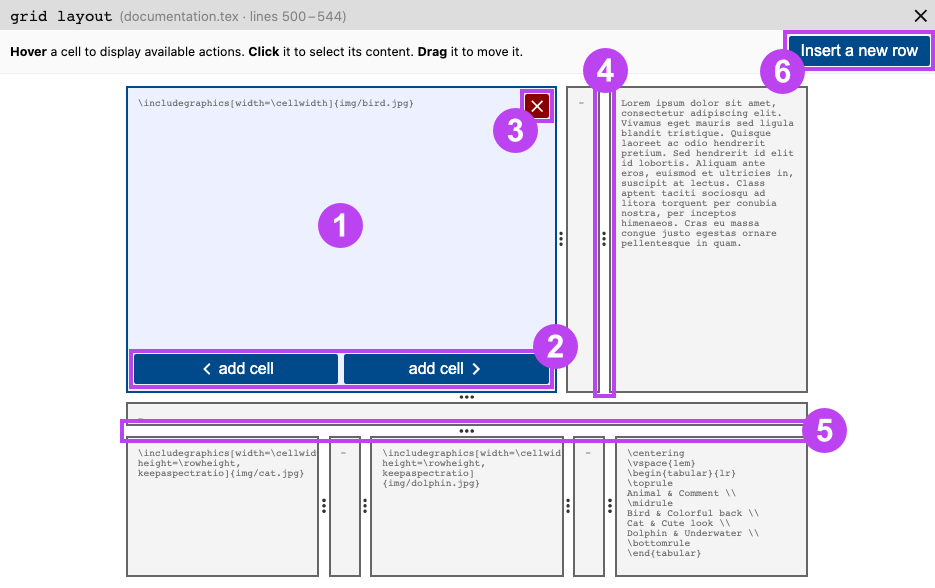
\includegraphics[width = 0.95\textwidth]{img/iir-gridlayout.png}
    \caption{The IIR of \texttt{gridlayout} environments. \figstep{1} A cell of the layout that is pointed by the mouse. It can be dragged to be moved before or after another cell. \figstep{2} Buttons to insert a new cell. \figstep{3} Button to remove the cell. \figstep{4} Separator between two cells. It can be dragged to resize the adjacent cells. \figstep{5} Separator between two rows. It can be dragged to resize the adjacent rows. \figstep{6} Button to insert a new row at the bottom of the grid.}
    \label{fig:iir-gridlayout}
\end{figure}

An IIR for grid layouts (\autoref{fig:iir-gridlayout}) can be created with the \texttt{gridlayout} environment.
A grid can contain rows (\texttt{row} environments), and a row can contain cells (\texttt{cell} environments).
A cell can contain \textbf{arbitrary content} (text, image, table, etc), but it \textbf{cannot contain} other special commands and environments provided by \iLaTeX{}!

\begin{lstlisting}[style=custom-latex]
% this grid is as wide as the text (\textwidth) and 8cm tall
\begin{gridlayout}{\textwidth}{8cm}
    \begin{row}{0.6}
        \begin{cell}{1}
            % A cell as wide as the row that contains it
        \end{cell}
    \end{row}
    \begin{row}{0.4}
        \begin{cell}{0.33}
            % Bottom-left cell taking 1/3 of the row
        \end{cell}
        \begin{cell}{0.67}
            % Bottom-right cell taking 2/3 of the row
        \end{cell}
    \end{row}
\end{gridlayout}
\end{lstlisting}

Contrary to the other IIRs, this IIR is not a wrapper around an existing command or environment.
Internally, every row and every cell is implemented as a \texttt{minipage}.

The \texttt{grid} environment expects two mandatory arguments: the \textbf{width} and the \textbf{height} of the grid.
The \texttt{row} and \texttt{cell} environments expect one mandatory argument each: the \textbf{relative height} of the row and the \textbf{relative width} of the cell. These relative dimensions are \textbf{unitless numbers between 0 and 1} that must sum to 1 over all the cells of a row and over all the rows of the grid.

\begin{info}
    In every cell, \iLaTeX{} defines \verb|\cellwidth| and \verb|\rowheight|, two custom length macros relative to the current size of the cell that you can freely use (\eg to make an image have the same width or height than the cell).
\end{info}

\begin{warning}
    You should always use at least one row with at least one cell in a \texttt{gridlayout} environment, and you should avoid putting anything outside of a \texttt{cell} environment.
    Doing so is likely to break the layout, and the IIR will not represent it correctly anymore.
\end{warning}

\begin{example}
    Try to click the layout below, to understand how it is built, and to edit it using the IIR.

    \begin{gridlayout}{\textwidth}{11cm}
        \begin{row}{0.65}
            \begin{cell}{0.646}
                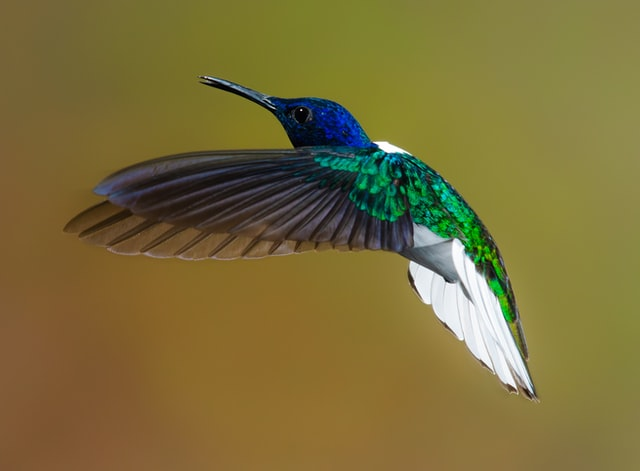
\includegraphics[width=\cellwidth]{img/bird.jpg}
            \end{cell}
            \begin{cell}{0.054}
                ~
            \end{cell}
            \begin{cell}{0.3}
                Lorem ipsum dolor sit amet, consectetur adipiscing elit. Vivamus eget mauris sed ligula blandit tristique. Quisque laoreet ac odio hendrerit pretium. Sed hendrerit id elit id lobortis. Aliquam ante eros, euismod et ultricies in, suscipit at lectus. Class aptent taciti sociosqu ad litora torquent per conubia nostra, per inceptos himenaeos. Cras eu massa congue justo egestas ornare pellentesque in quam.
            \end{cell}
        \end{row}
        \begin{row}{0.05}
            \begin{cell}{1}
                ~ 
            \end{cell}
        \end{row}
        \begin{row}{0.3}
            \begin{cell}{0.3}
                
\includegraphics[width=\cellwidth, height=\rowheight, keepaspectratio]{img/cat.jpg}
            \end{cell}
            \begin{cell}{0.05}
                ~
            \end{cell}
            \begin{cell}{0.3}
                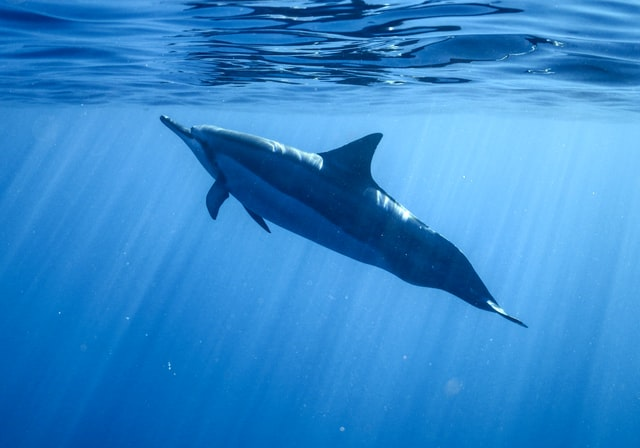
\includegraphics[width=\cellwidth, height=\rowheight, keepaspectratio]{img/dolphin.jpg}
            \end{cell}
            \begin{cell}{0.05}
                ~
            \end{cell}
            \begin{cell}{0.3}
                \centering
                \vspace{1em}
                \begin{tabular}{lr}
                    \toprule
                    Animal & Comment \\
                    \midrule
                    Bird & Colorful back \\
                    Cat & Cute look \\
                    Dolphin & Underwater \\
                    \bottomrule
                \end{tabular}
            \end{cell}
        \end{row}
    \end{gridlayout}
\end{example}






%%%%%%%%%%%%%%%%%%%%%%%%%%%%%%%%%%%%%%%%%%%%%%%%%%%%
%%%%%%%%%%%%%%%%%%%%   DEMO 1   %%%%%%%%%%%%%%%%%%%%
%%%%%%%%%%%%%%%%%%%%%%%%%%%%%%%%%%%%%%%%%%%%%%%%%%%%

\largetitle{Exercise and demo}

% Images taken from https://arxiv.org/abs/2103.10428
\taskone

\begin{task}
%%%%%%%%%%%%%%%%%%%%%%%%%%%%%%%% START EDITING HERE
    \begin{gridlayout}{\textwidth}{12cm}
        \begin{row}{0.33}
            \begin{cell}{0.25}
                \centering
                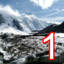
\includegraphics[width=0.9\cellwidth]{img/thumbnail-1.png}
            \end{cell}
            \begin{cell}{0.25}
                \centering
                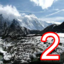
\includegraphics[width=0.9\cellwidth]{img/thumbnail-2.png}
            \end{cell}
            \begin{cell}{0.25}
                \centering
                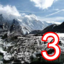
\includegraphics[width=0.9\cellwidth]{img/thumbnail-3.png}
            \end{cell}
            \begin{cell}{0.25}
                \centering
                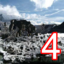
\includegraphics[width=0.9\cellwidth]{img/thumbnail-4.png}
            \end{cell}
        \end{row}
        \begin{row}{0.33}
            \begin{cell}{0.25}
                \centering
                
\includegraphics[width=0.9\cellwidth]{img/thumbnail-5.png}
            \end{cell}
            \begin{cell}{0.25}
                \centering
                
\includegraphics[width=0.9\cellwidth]{img/thumbnail-6.png}
            \end{cell}
            \begin{cell}{0.25}
                \centering
                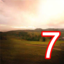
\includegraphics[width=0.9\cellwidth]{img/thumbnail-7.png}
            \end{cell}
            \begin{cell}{0.25}
                \centering
                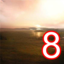
\includegraphics[width=0.9\cellwidth]{img/thumbnail-8.png}
            \end{cell}
        \end{row}
        \begin{row}{0.34}
            \begin{cell}{0.25}
                \centering
                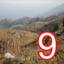
\includegraphics[width=0.9\cellwidth]{img/thumbnail-9.png}
            \end{cell}
            \begin{cell}{0.25}
                \centering
                
\includegraphics[width=0.9\cellwidth]{img/thumbnail-10.png}
            \end{cell}
            \begin{cell}{0.25}
                \centering
                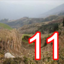
\includegraphics[width=0.9\cellwidth]{img/thumbnail-11.png}
            \end{cell}
            \begin{cell}{0.25}
                \centering
                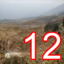
\includegraphics[width=0.9\cellwidth]{img/thumbnail-12.png}
            \end{cell}
        \end{row}
    \end{gridlayout}
%%%%%%%%%%%%%%%%%%%%%%%%%%%%%%%% STOP EDITING HERE
\end{task}

\newpage






%%%%%%%%%%%%%%%%%%%%%%%%%%%%%%%%%%%%%%%%%%%%%%%%%%%%
%%%%%%%%%%%%%%%%%%%%   DEMO 2   %%%%%%%%%%%%%%%%%%%%
%%%%%%%%%%%%%%%%%%%%%%%%%%%%%%%%%%%%%%%%%%%%%%%%%%%%

\newpage

% Top
\centering
Internship report

\vspace{3cm}

\rule{0.6\textwidth}{0.4pt}\\[1.5ex]
{\Large Internship title}\\
\rule{0.6\textwidth}{0.4pt}

\vspace{6cm}

\textbf{Firstname \textsc{Lastname}} \\
supervised by Firstname \textsc{Lastname}

\vfill

\begin{gridlayout}{\textwidth}{5cm}
    \begin{row}{0.5}
        \begin{cell}{0.25}
            \centering
            
\includegraphics[width=\cellwidth, height=\rowheight, keepaspectratio]{img/logo-inria.png}
        \end{cell}
        \begin{cell}{0.125}
            ~ % Separator
        \end{cell}
        \begin{cell}{0.25}
            \centering
            
\includegraphics[width=\cellwidth, height=\rowheight, keepaspectratio]{img/logo-cnrs.png}
        \end{cell}
        \begin{cell}{0.125}
            ~ % Separator
        \end{cell}
        \begin{cell}{0.25}
            \centering
            
\includegraphics[width=\cellwidth, height=\rowheight, keepaspectratio]{img/logo-inserm.png}
        \end{cell}
    \end{row}
    \begin{row}{0.5}
        \begin{cell}{0.1}
            ~ % Separator
        \end{cell}
        \begin{cell}{0.25}
            \centering
            
\includegraphics[width=\cellwidth, height=\rowheight, keepaspectratio]{img/logo-ex-situ.png}
        \end{cell}
        \begin{cell}{0.3}
            ~ % Separator
        \end{cell}
        \begin{cell}{0.25}
            \centering
            
\includegraphics[width=\cellwidth, height=\rowheight, keepaspectratio]{img/logo-univ-ps.png}
        \end{cell}
        \begin{cell}{0.1}
            ~ % Separator
        \end{cell}
    \end{row}
\end{gridlayout}



\end{document}